
不关心设备代码在哪里运行时,可以让运行时库帮忙选择。这种自动选择是不关心选择了什么设备时,可以很容易地开始编写和运行代码。这种设备选择没有考虑要运行的代码特性,所以是一个随意的选择,这个选择很可能不是最优的。\par

讨论设备的选择(即使是实现为选择的设备)之前,应该首先讨论与设备交互的机制:\textbf{队列}。\par

\hspace*{\fill} \par %插入空行
\textbf{队列}

队列是一种抽象,将操作提交给它在单个设备上执行。图2-3和图2-4给出了\textit{queue}类的定义。入队的通常是数据并行的计算,当需要更多的控制时,也可以使用其他命令,如手动控制数据移动。提交到队列的工作需要满足运行时跟踪的先决条件(例如输入数据的可用性)进行执行。这些先决条件在第3章和第8章中有介绍。\par

\hspace*{\fill} \par %插入空行
图2-3 简化的queue类
\begin{lstlisting}[caption={}]
class queue {
public:
	// Create a queue associated with the default device
	queue(const property_list = {});
	queue(const async_handler&, 
		  const property_list = {});
	
	// Create a queue associated with an explicit device
	// A device selector may be used in place of a device
	queue(const device&, const property_list = {});
	queue(const device&, const async_handler&, 
	      const property_list = {});
	
	// Create a queue associated with a device in a specific context
	// A device selector may be used in place of a device
	queue(const context&, const device&, 
		  const property_list = {});
	queue(const context&, const device&, 
		  const async_handler&, 
		  const property_list = {});
};
\end{lstlisting}

\hspace*{\fill} \par %插入空行
图2-4 简化了queue类中的关键成员函数
\begin{lstlisting}[caption={}]
class queue {
public:
	// Submit a command group to this queue.
	// The command group may be a lambda or functor object.
	// Returns an event representation the action 
	// performed in the command group.
	template <typename T>
	event submit(T);
	
	// Wait for all previously submitted actions to finish executing.
	void wait();
	
	// Wait for all previously submitted actions to finish executing.
	// Pass asynchronous exceptions to an async_handler if one was provided.
	void wait_and_throw();
};
\end{lstlisting}	
	
队列绑定到单个设备,绑定发生在队列的构造过程中。提交给队列的工作是在该队列绑定的设备上执行的。队列不能映射到设备集合,因为这会不明确应该在哪个设备上执行工作。同样,队列也不能将提交的工作分散到多个设备上。相反,队列和提交给队列的工作将在执行设备之间有一个明确的映射,如图2-5所示。\par

\hspace*{\fill} \par %插入空行
图2-5 队列绑定到单个设备,提交到队列中的工作在相应的设备上执行
\begin{center}
	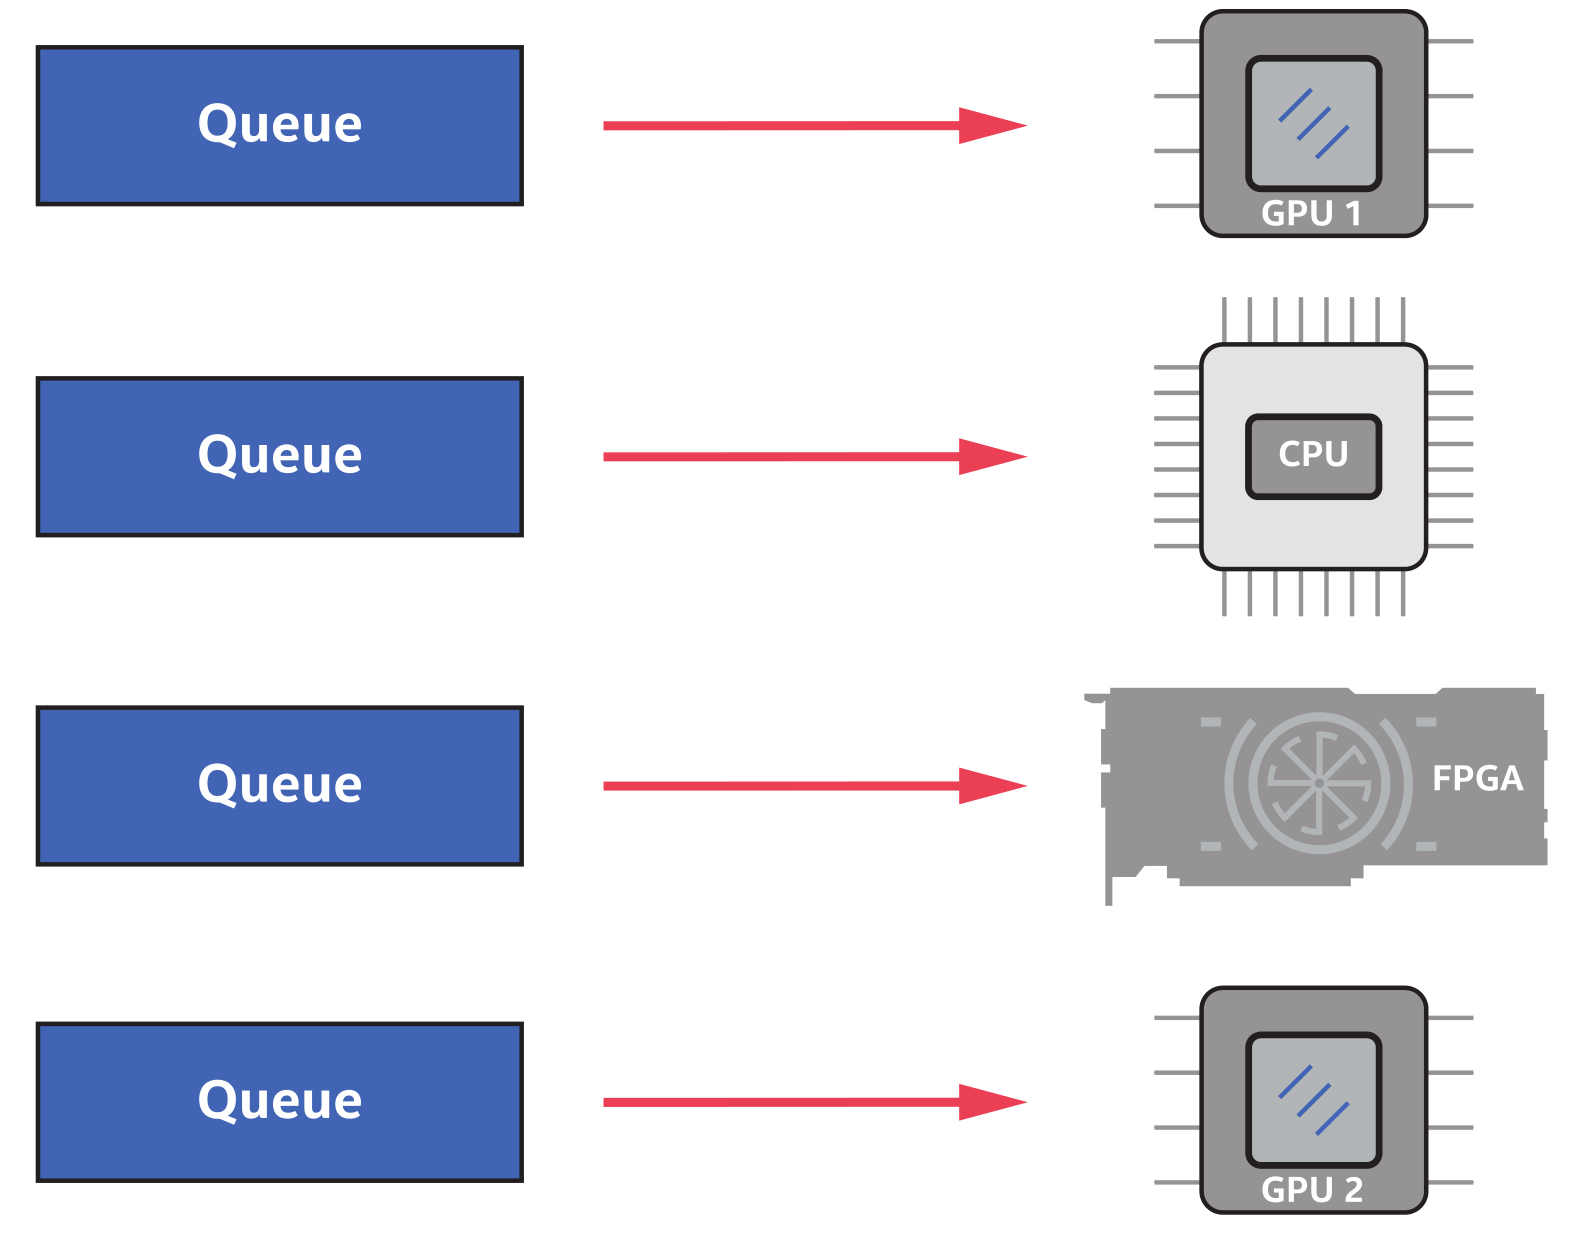
\includegraphics[width=1.\textwidth]{content/chapter-2/images/4}
\end{center}

程序中可以创建多个队列,让每个队列与不同的设备绑定,或者让主机中的不同线程使用。多个不同的队列可以绑定到单个设备上,提交到这些不同队列的工作将组合在设备上执行,如图2-6所示。相反,正如我们前面提到的,队列不能绑定到多个设备,因为在执行操作的位置上不能有任何歧义。例如,想要一个能够跨多个设备加载平衡工作的队列,需要先创建这个对象。\par

\hspace*{\fill} \par %插入空行
图2-6 多个队列可以绑定到单个设备
\begin{center}
	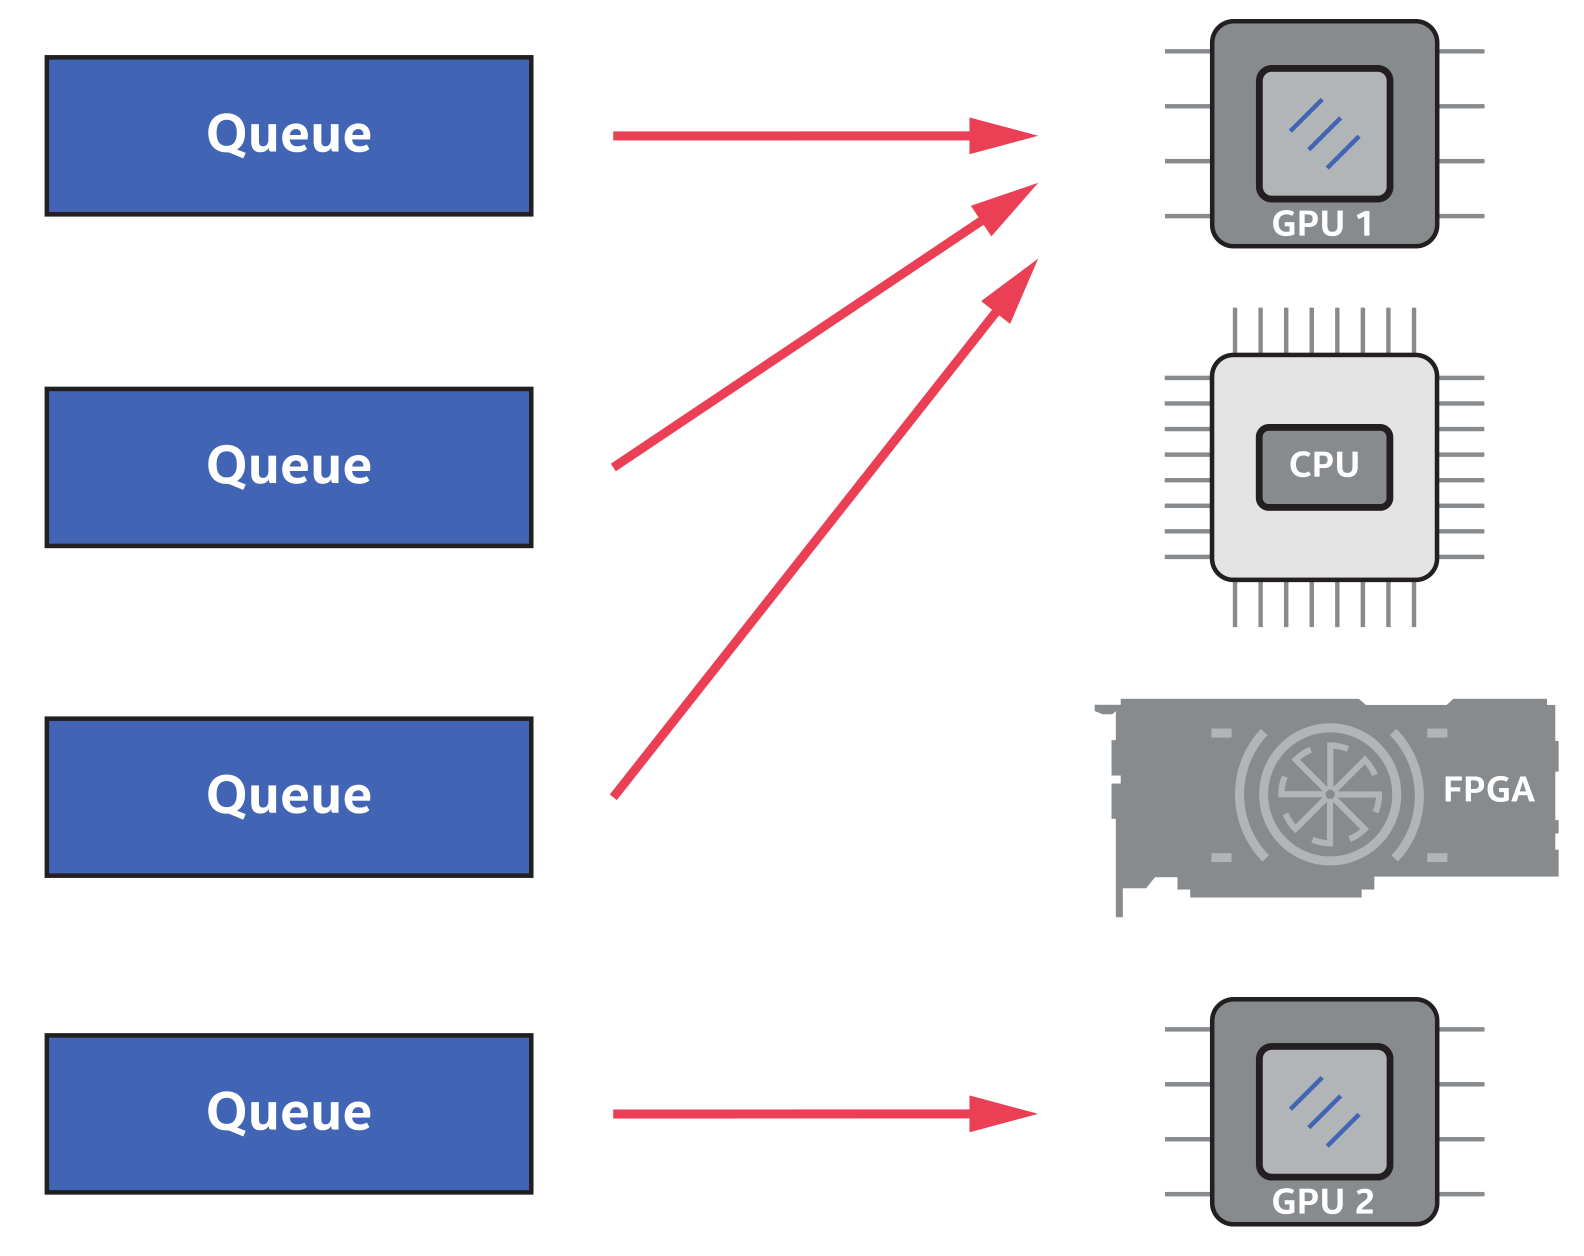
\includegraphics[width=1.\textwidth]{content/chapter-2/images/5}
\end{center}

因为队列绑定到特定的设备,所以提交给队列的操作是将相应工作在设备上执行的常用方法。构造队列时选择设备是通过设备选择器和\textit{device\_selector}类实现的。\par

\hspace*{\fill} \par %插入空行
\textbf{绑定队列与设备(任何设备都可以)}

图2-7是没有指定队列绑定设备的示例。queue的构造函数没有任何参数(如图2-7所示),只是选择一些可用的设备。SYCL保证至少有一个设备可用,即主机。主机也可以运行内核代码,它是执行主机程序的处理器,所以总是存在。\par

\hspace*{\fill} \par %插入空行
图2-7 通过队列的隐式构造,选择默认设备
\begin{lstlisting}[caption={}]
#include <CL/sycl.hpp>
#include <iostream>
using namespace sycl;

int main() {
	// Create queue on whatever default device that the implementation
	// chooses. Implicit use of the default_selector. 
	queue Q;
	
	std::cout << "Selected device: " <<
	Q.get_device().get_info<info::device::name>() << "\n";
	
	return 0;
}

Possible Output:
Device: SYCL host device
\end{lstlisting}	

使用queue的构造函数是启动设备代码的最简单方法。对于绑定到队列的设备的选择,因为与我们的应用程序相关,可以添加更多的控制。\par













